% !TeX root = ../../../main.tex
\begin{figure}[htbp]
\begin{ChFiveFloatBody}
    \centering
    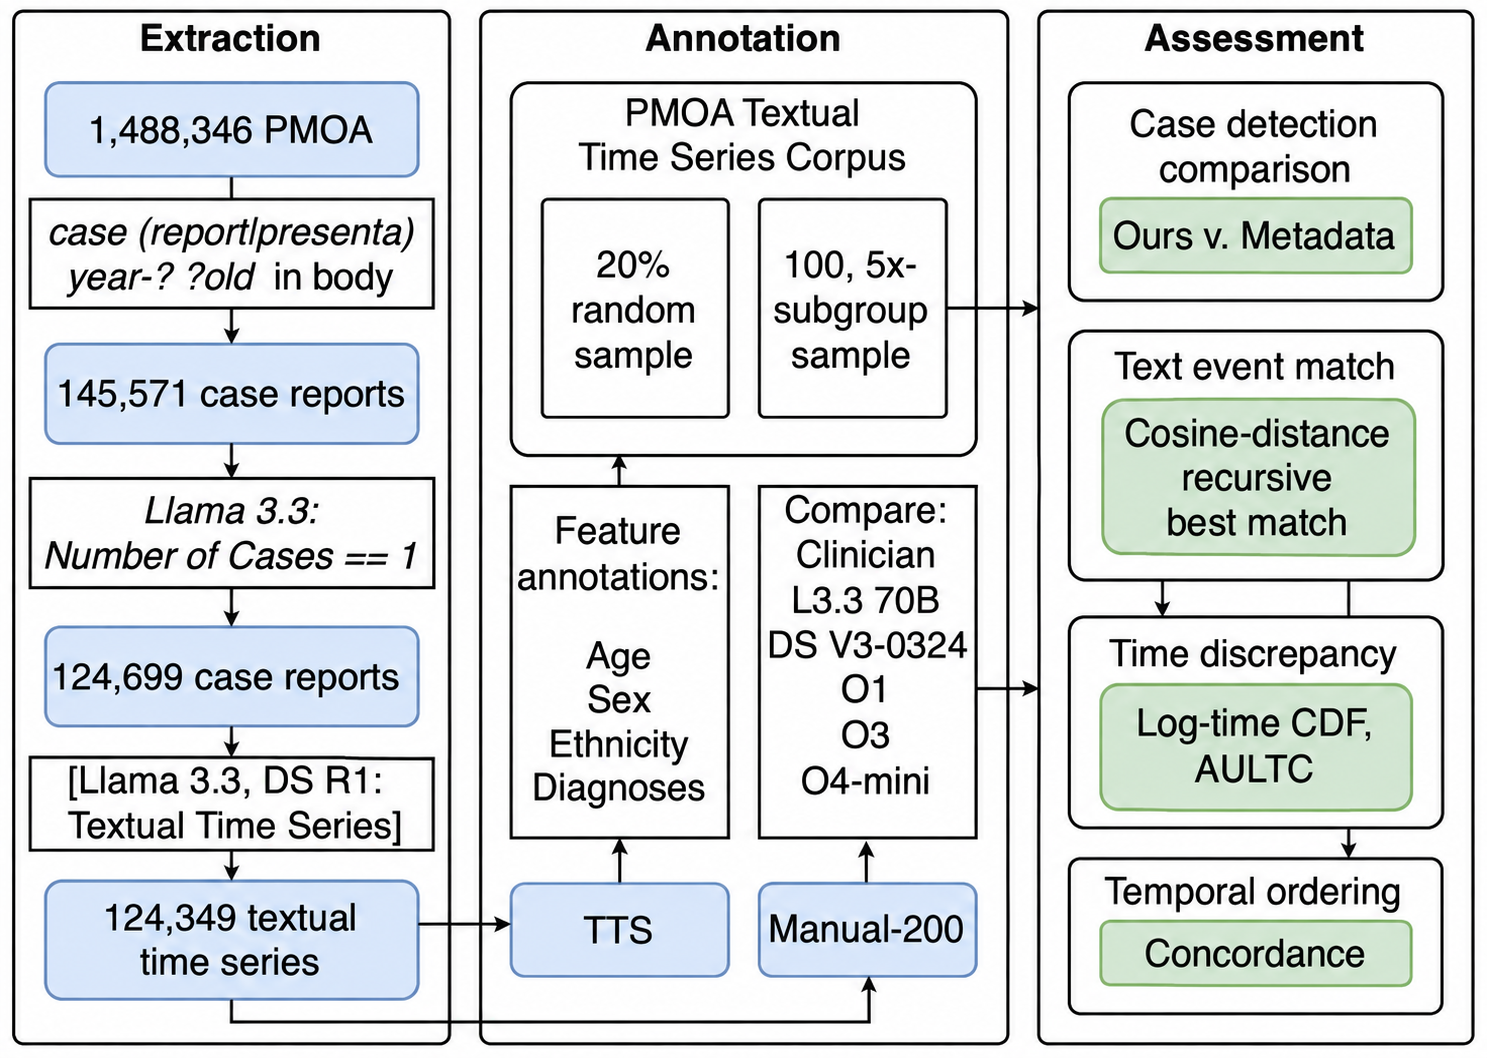
\includegraphics[width=0.75\linewidth]{Chapters/chapter-05/images/Scientific_data/Plots_tables/PMOATTS_flow5_v2.png} %
    
    
    

\end{ChFiveFloatBody}
\caption{Flowchart of the extraction and annotation pipeline. The left panel (Extraction) shows how we filtered the PMOA corpus to identify single-patient case reports. The middle panel (Annotation) depicts the generation of textual time series for each case via LLM prompting and the creation of evaluation subsets. The right panel (Assessment) summarizes the evaluation process, including metadata comparison, text event matching, time discrepancy analysis (log-time CDF, AULTC), and temporal order concordance.
    }\ChFiveFloatLabel{ch05:fig:flowchart}
\end{figure}